
\chapter{Simulation Time Delay Tele-operation}
\label{c7_DI_equimomental}
In this chapter simulation of a teleoperated mobile platform is presented. In tele-operation the human operators observe a remote scene through camera/s, and manipulating the local steering wheel and accelerator paddle as shown in figure \ref{fig:teleoperation} . The command is transmitted to the mobile robot over wireless network. The operator response is based on the latest feedback images from the cameras. The simulation results are presented of robots behaviour for the delayless and delay transmission network.
\begin{figure}
	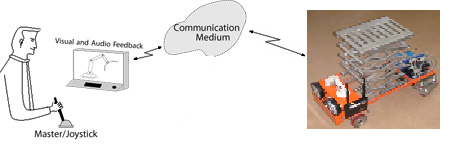
\includegraphics[width=\linewidth,keepaspectratio]{Chapter6/fig/teleoperation}
	\captionof{figure}{Teleoperation  Architecture }
	\label{fig:teleoperation} 
\end{figure}

\section{Tele operation simulation architecture}
The standard kinematic model as described in \cite{campion1996structural} of the mobile platform is used for the simulation. This is justified as  the vehicle is expected to move at relatively slow speed. The inputs to the model are the left and right rear wheel velocities. The front wheels are steered to satisfy the Ackerman condition as presented in **** and are assumed to attain the desired angle instantaneously. Therefore the robot can be treated as differential drive robot.  The kinematic model of the platform is presented below
\begin{equation}
\begin{pmatrix}
\dot{x}\\ 
\dot{y}\\ 
\dot{\theta}
\end{pmatrix}
=
\begin{pmatrix}
\sin \theta & 0 \\
-\cos \theta & 0 \\
0& 1
\end{pmatrix}
\begin{pmatrix}
r/2 & r/2\\
1/b & -1/b
\end{pmatrix}
\begin{pmatrix}
\dot{\phi_L}\\
\dot{\phi_R}
\end{pmatrix}
\end{equation}


Where ,  $b$is the distance between the rear wheels,$r$ wheel radius. $\dot{\phi_R}$ and $\dot{\phi_L} $ are the left and right wheel rotational velocity. 

The operator station sends the command $u_1$ and $u_2$ over the wireless network, in general it will be delayed by $\delta$ time. These commands are interpreted by the robot controller as the left and right wheel velocities.  Therefore by taking the time delay into consideration we can write
\begin{equation}
\begin{pmatrix}
\dot{\phi_R}(t) \\
 \dot{\phi_L}(t)
\end{pmatrix}
=
\begin{pmatrix}
u_1(t-\delta)\\
u_1(t-\delta)
\end{pmatrix}
\end{equation}

The control inputs to the mobile robot  $u_1$ and $u_2$ are generate by the operator based on the visual data available to him. We next present the model of the human operator to be used for simulation the complete loop.


\section{Modeling the human operator}
In order to simulate the teleoperation loop we need a mathematical model of human operator. The mathematical  modelling of the operator`s action is modelled assuming a car driving metaphor. The video feedback, which the he receives of the remote environment, give him the idea of the vehicles  position and the tentative next goal point (p) based on a lookahead distance (l). He then constructs a  virtual path mentally and tries to manoeuvre or steers the robot to follow that path as shown in figure \ref{fig:drivingStratagy}. As he moves forward the goal point keeps changing until he reaches the desired location. This methodology of path tracing is known as pure pursuit \cite{coulter1992implementation} or following the carrot strategy. 
\begin{figure}
	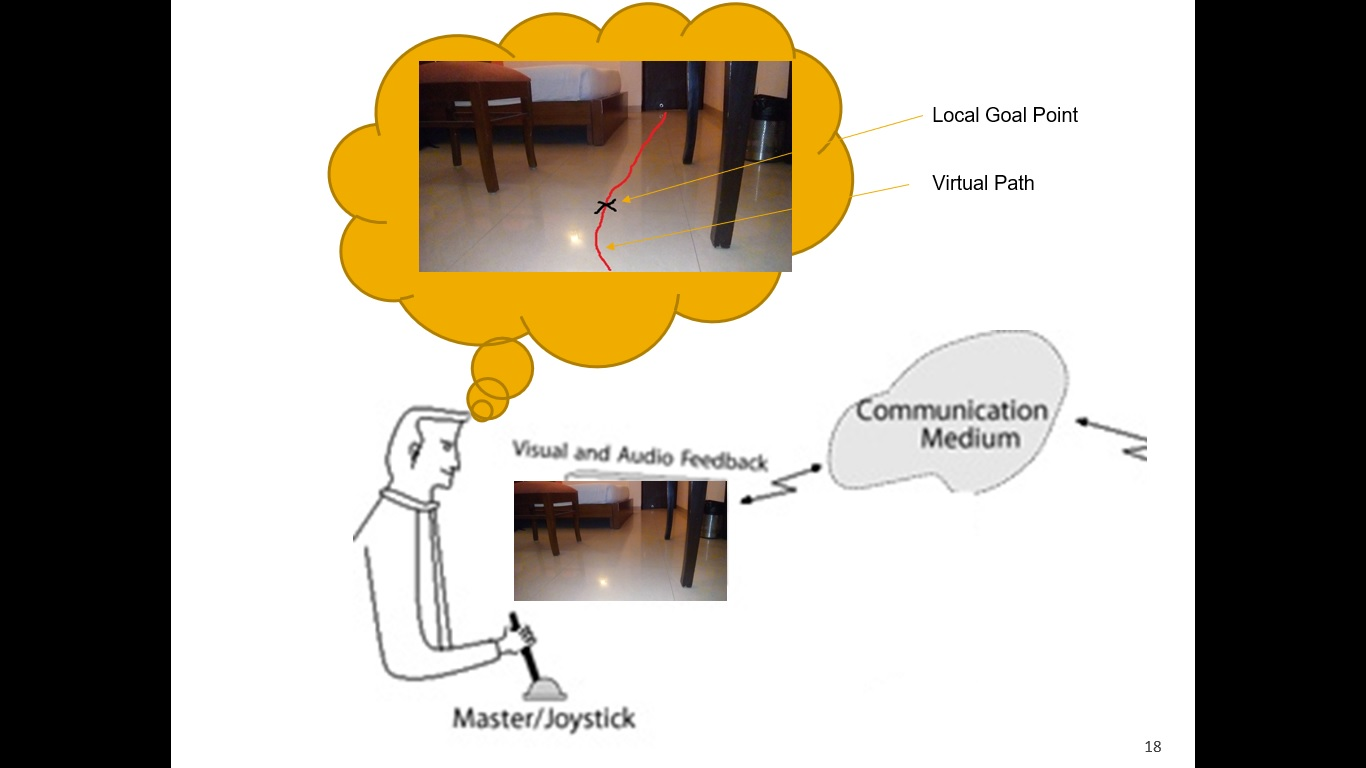
\includegraphics[width=\linewidth,keepaspectratio]{Chapter6/fig/mentalMap}
	\captionof{figure}{Assumed driving strategy  }
	\label{fig:drivingStratagy} 
\end{figure}

The mathematical model is derived next.

\section{Simulation Results }
\section{Predictive Model based Feedback}
\subsection{Using Dynamic model of vehicle}
\subsection{Kalman Filter with odometer data and Accelorometer?}


\section{Summary}
In this chapter, 